\documentclass[11pt]{wbzine}
%packages
\usepackage{lipsum}
\usepackage[utf8]{inputenc}
\usepackage[T1]{fontenc}
\usepackage[ngerman]{babel}
\usepackage{coelacanth}
%\usepackage{imfellEnglish}
%\renewcommand*\sfdefault{ugq}


\begin{document}

\begin{titlepage}
\centering
{\bfseries\fontsize{70}{55}\selectfont Grenzland}

\hrulefill Jahrgang 1, Heft 1, August 2022
    \vspace{1cm}

	  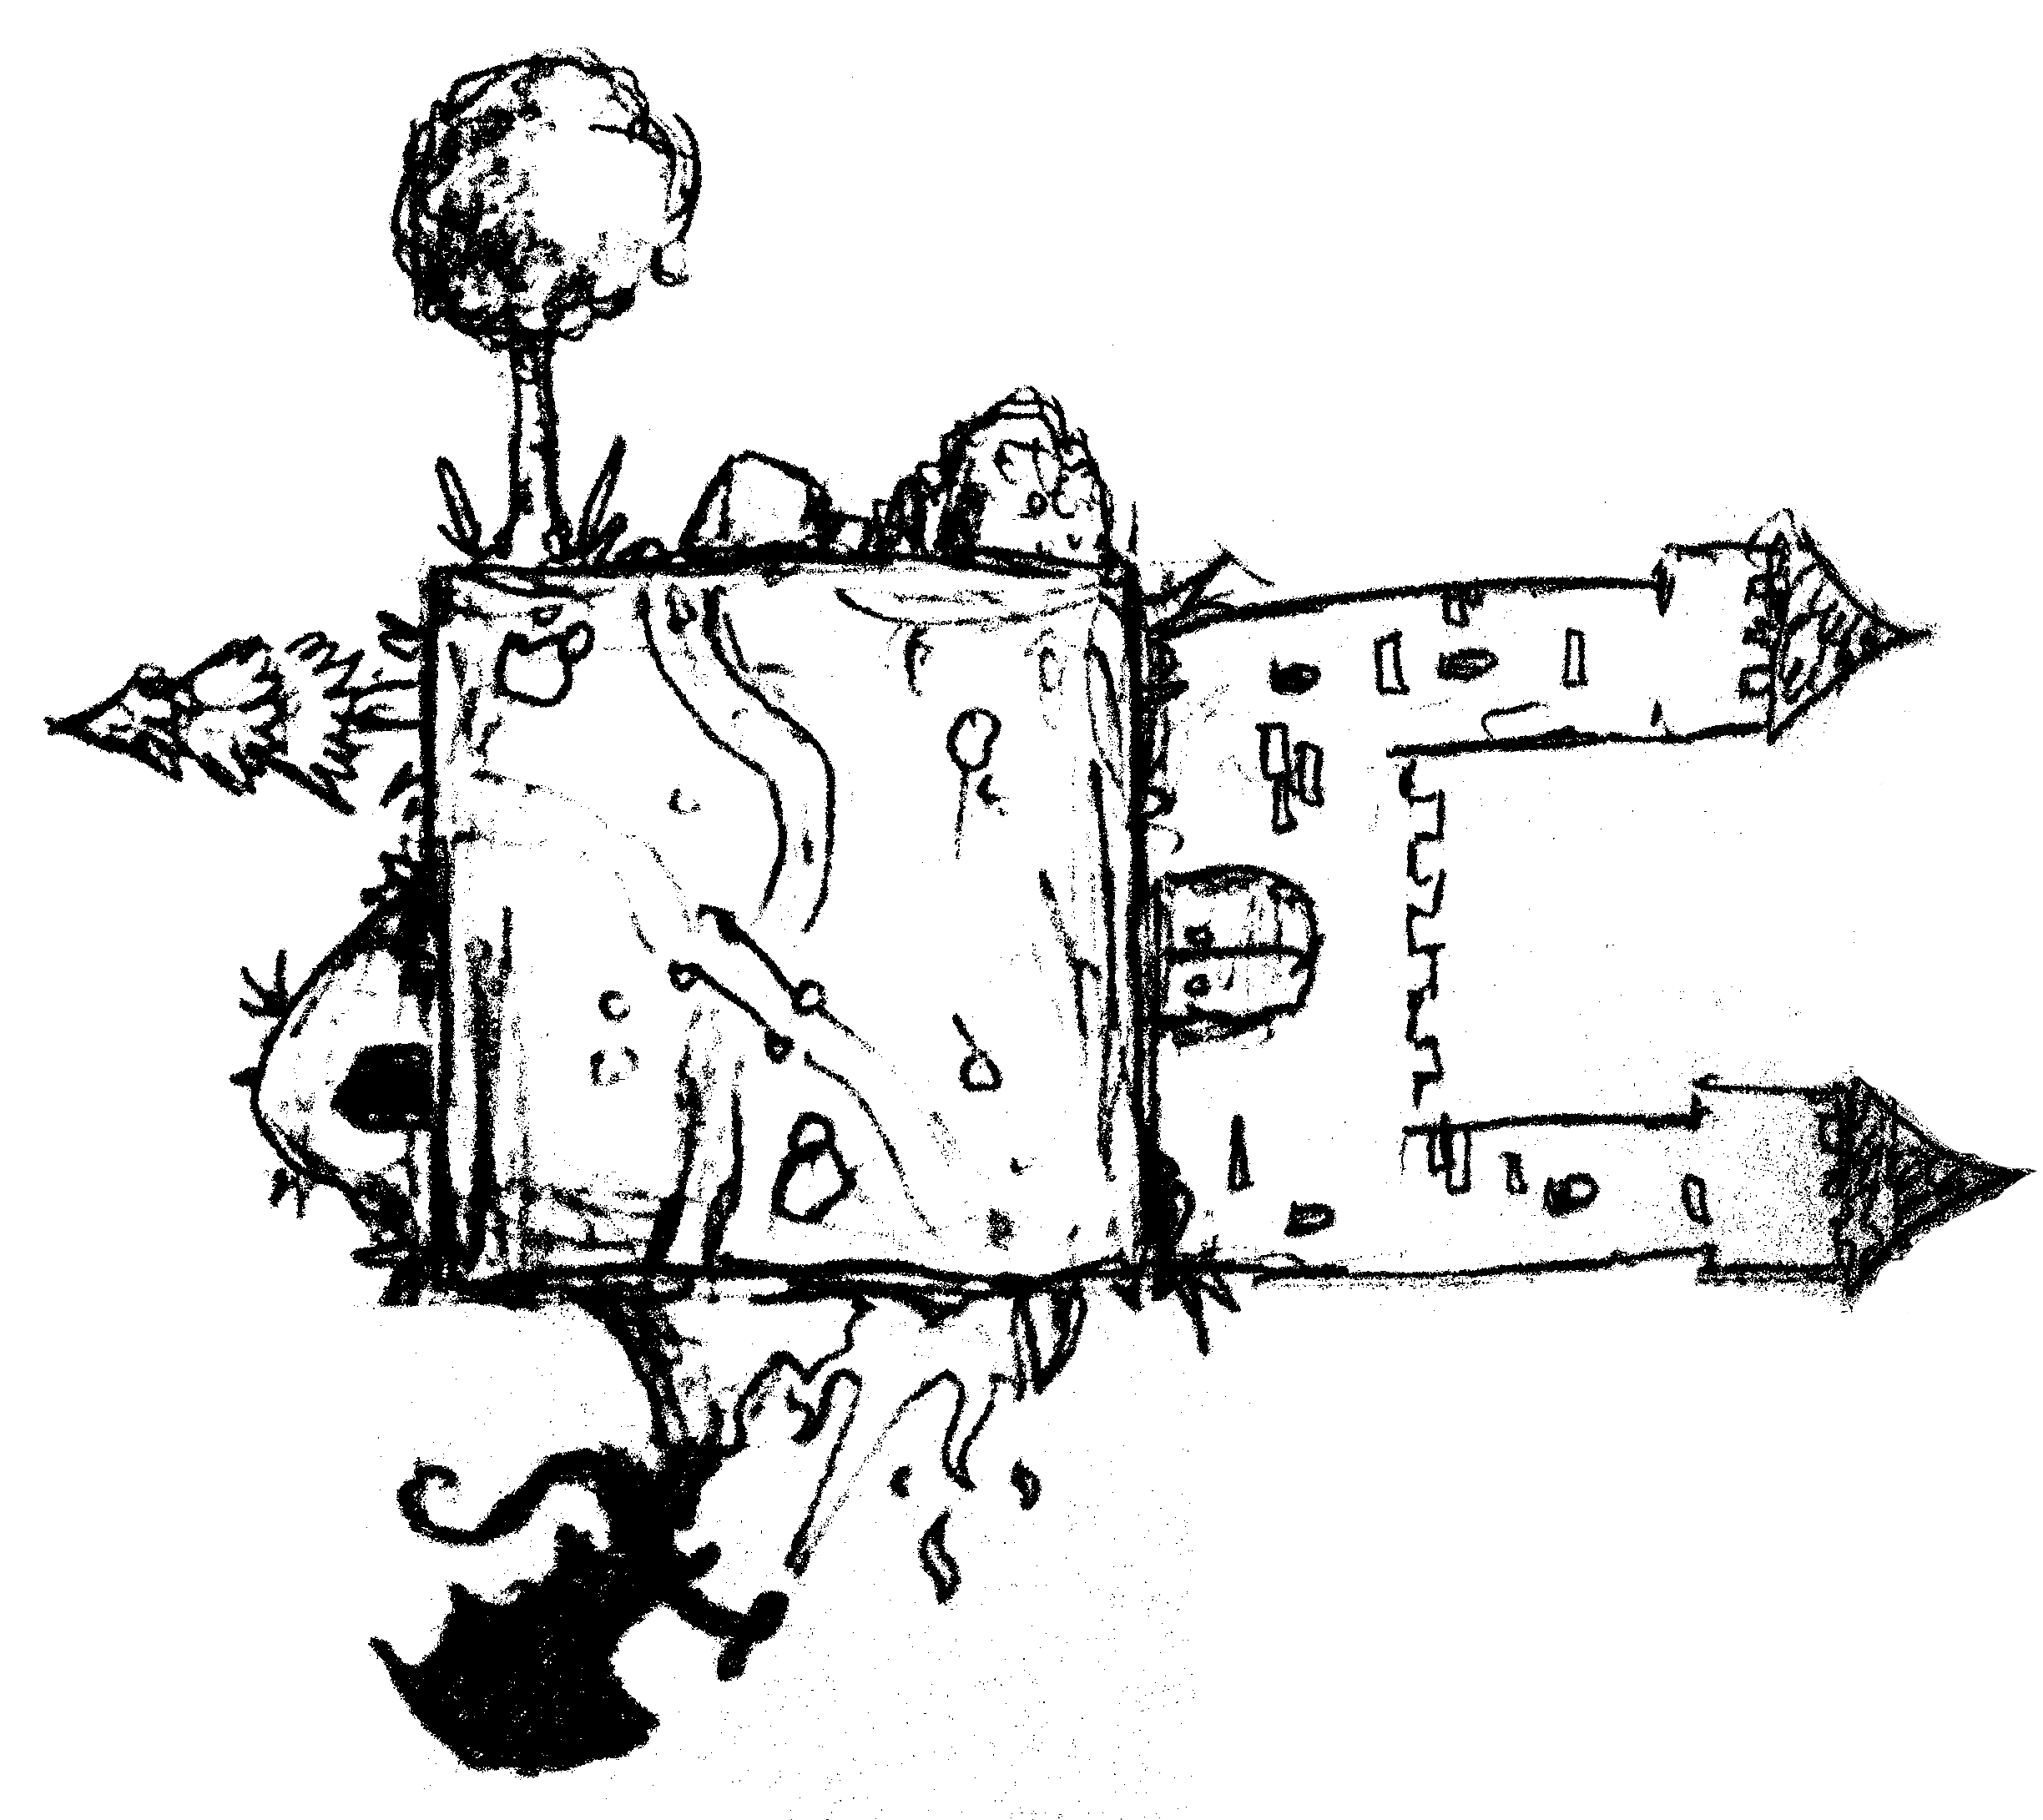
\includegraphics[width=\textwidth]{Coverimage.png}

    \vspace{1cm}
{\Huge Nach dem Kataklysmus\par}%

\end{titlepage}

\tableofcontents

\begin{multicols}{2}

\section{Vorwärts!}
\by{DM Laurens}

Die erste Session der Grenzland-Kampagne wurde am 08.04.2016
    gespielt, die letzte am 23.04.2021. Über diese 5 Jahre spielten
    wir rund 50 Sessions. Zu Beginn in monatlichen Abständen, später
    alle 2 Wochen, und seit Anfang 2021 wöchentlich – immer mit
    einer Sommerpause von Ende April bis Ende September. Rund 20
    Spieler:innen beteiligten sich in wechselnder Konstellation an
    der Kampagne. Rund 30 Charaktere starben im Verlauf der Kampagne
    … oh boy … Die alten D\&D Varianten sind berühmt und berüchtigt
    für ihre ``Tödlichkeit''.

Nun soll es also wieder los gehen. Die Katastrophe, mit der das alte
    Grenzland endete, bietet jetzt, fast zwei Jahre später ein paar
    großartige Anknüpfungspunkte, und löst gleichzeitig ein paar
    Probleme, die ich mit der Kampagnenwelt hatte. Während das alte
    Grenzland auf der veröffentlichten Welt \textit{Mystara}
    beruhte, die viele Ungereimtheiten und einen quasi fest
    geschriebenen Kanon hat, ist das postapokalymptische Grenzland
    neu, anders, und plötzlich etwas eigenes. Und das
    postapokalyptische Grenzland ist nun auch eindeutig unsere Erde
    vor langer langer Zeit. 


Dann also: auf die nächsten 5 Jahre Grenzland!

\section{Was bisher geschah}

Zu Beginn spielten sich die Ereignisse der Kampagne zwischen der
    Festung im Grenzland und den Chaoshöhlen ab. Die Charaktere
    waren ins Grenzland gekommen, um auf Abenteuer auszuziehen, und
    so Ruhm und Gold zu gewinnen. Nicht wenige Charaktere bezahlten
    das mit ihrem Leben, und noch mehr Monster in den Wäldern und
    Höhlen mussten dran glauben. Schließlich überfiel der mächtige
    Drache Darpantor die Festung und die Charaktere waren gezwungen
    die Festung zu verlassen. Sie fanden Zuflucht im zwei
    Tagesreisen westlich gelegenen Hommlet und zogen fortan von dort
    auf Abenteuer aus. Zu Beginn auch noch gelegentlich in die
    Ruinen der Festung, die nun von Dämonen heimgesucht wurde.

Später – in der 4. Spielzeit – begab man sich auf eine Reise in das
    Reich der Zwerge im nördlichen Gebirge. Das Ziel war,
    Handelsbeziehungen mit den Zwergen aufzubauen, und andererseits
    einem der Spielercharaktere bei der Erfüllung ihrer Queste zu
    helfen. Am Ende wurde so ein von dunklen Mächten gefangener
    Golddrache – der ``irdische'' Avatar einer rechtschaffenen
    Gottheit – von den Spielercharakteren befreit, und das Land der
    Zwerge vor dem Verderben bewahrt. 

\bigmap{Grenzland-praeapo.png}


    Schließlich trat mit der 5. Spielzeit ein seltsamer Kult auf den
    Plan. Die ``Einmonder'' – fanatisch rechtschaffene Kleriker und
    Zauberkundige aus der königlichen Hauptstadt – hatten sich in den
    Kopf gesetzt, einen der beiden Monde, den roten Mond
    Daro aus dem Himmel zu heben, um dadurch dem Chaos ein für alle
    mal Einhalt zu gebieten. Am Ende stellte sich heraus, dass alles
    eine Verschwörung des Drachen Darpantor war. Er hatte 50 Jahre
    zuvor mit einem anderen Drachen gewettet, dass es ihm gelingen
    würde Daro aus dem Himmel zu heben.

    Allein, Darpantor verlor am Ende seine Wette. Den
    Spielercharakteren gelang es zwar nicht, die Einmonder an der
    Durchführung ihres wahnsinnigen Rituals zu hindern, doch sie
    konnten so viel Verwirrung stiften, dass es am Ende Maro, den
    anderen, helleren der beiden Monde traf. Selbst Darpantor, der
    die Wut über sein Scheitern an den Helden auslassen wollte,
    konnte in die Flucht geschlagen werden. Schließlich, durch das
    Zerreißen des Mondes, erschütterten heftige Erdbeben das
    Grenzland, tiefe Erdspalten rissen auf, und verschluckten so
    manchen Abenteurer für immer. Andere wurden auf fremde Ebenen
    gerissen, und nur wenige konnten später von den letzten Tagen
    des alten Grenzlandes berichten.

\subsection{Nach dem Kataklysmus}

Über viele Monate erschütterten immer neue Erdbeben das Grenzland,
und herabstürzende Fragmente des zerstörten Mondes liessen das Land
nicht zur Ruhe kommen. Dicke Staubwolken verdunkelten den Himmel,
und führten zu einer monatelang anhaltenden, eiskalten Nacht. Bis
heute sind große Teile des ehemaligen Grenzlandes unter einer viele
Meter dicken Schicht aus Schutt und grauem Schnee begraben.

Weite Teile des Landes sind durch das Aufbersten gewaltiger Gräben
für immer verändert, und große Teile der Küstenregionen sind für
immer im Meer versunken. Das alte Königreich, das Imperium im Osten,
und die große Wüste sind für immer verschwunden. Dort wo über
Jahrtausende der alte Elfenwald war, zieht ein riesiger Fjord weit
ins Landesinnere.

Versprengte Gruppen überlebender Völker des alten Grenzlandes ziehen
durch die unwegsamen eiskalten Einöden, auf der Suche nach Nahrung,
Überresten der alten Zivilisation und grüneren Weiden hinter dem
Horizont. Das Leben ist rauh und gefährlich. Gelegentlich können
wertvolle Überreste der alten Zeit gefunden werden, doch die
zahlreichen tiefen Risse in der Erde bergen auch unergründete
Geheimnisse, und Dinge, die seit Äonen unter dem Sediment
der Zeit verborgen waren.

Auch die Inseln des Südens wurden während der letzten Monate immer
wieder von Erdbeeben und Tsunamis heimgesucht, doch die meisten
Menschen haben hier, weit weg vom Epizentrum der Katastrophe,
überlebt. Man sagt die Reiche des alten Festlandes, seien unter den
Trümmern der eigenen Hybris begraben, und junge Menschen machen sich
nun auf, die veränderte Welt neu zu entdecken. Irgendwo weit im
östlichen Ozean, so heißt es, soll gar eine neue Insel geboren
worden sein.

\bigmap{Grenzland-postapo.png}

\section{Neue Charaktere}

Charaktere werden nach den üblichen Regeln aus den 3 kleinen
Heftchen von 1974, bzw. nach Wanderer Bills \textit{Menschen \&
Magie, Spielerhandbuch} erzeugt. Mit jeweils 3W6 wird für folgende
Attribute gewürfelt: 

\begin{tabularx}{\columnwidth}{Zc}
    Stärkte & ST \\
    Intelligenz & IN \\
    Weisheit & WE \\
    Geschicklichkeit & GE \\
    Konstitution & KO \\
    Charisma & CH \\
\end{tabularx}

    Es gelten folgende Modifikatoren: 

\begin{tabularx}{\columnwidth}{cZ}
    ST & Effekt \\
    15+ & Erfahrungsbonus 10\% \\
    7- & Erfahrungsbonus -5\% \\
\end{tabularx}

\begin{tabularx}{\columnwidth}{cZ}
    IN & Effekt \\
    15+ & Erfahrungsbonus 10\% \\
    7- & Erfahrungsbonus -5\% \\
\end{tabularx}

\subsection{Charakterspezies}

Auf dem Festland gibt es die üblichen Spezies: Menschen, Elfen,
Zwerge und Halblinge. Die meisten Charaktere werden Menschen sein.
Wenn Du einen ``Halbmenschen'' spielen möchstest, überlege Dir gut,
warum, und mache den Unterschied zu Menschen im Rollenspiel
deutlich!

\subsection{Charakterklassen}

Grundsätzlich sind die üblichen drei Standardklassen möglich:
Krieger, Kleriker, und Zauberkundige. Allerdings starten neue
Charaktere auf Stufe 0 und noch ohne Klasse. In den ersten
Abenteuern wird sich zeigen, in welche Richtung Dein neuer Charakter
strebt. Wird er mit Waffen trainieren, und sich einem Söldnertrupp
anschließen? sich einer Glaubensgemeinschaft anschließen, und ein
Gelübte ablegen? Oder wird Dein Charakter sich als Lehrling bei
einem Meister der arkanen Wissenschaften verdingen?

Alle Charaktere starten mit 1W6 Trefferpunkten. Wenn sich Dein
Charakter für eine Klasse entschieden hat, kannst Du die
Trefferpunkte entsprechend der Klasse noch einmal neu würfeln, und
den höheren Wert behalten.

\end{multicols}

\begin{tabularx}{\textwidth}{crcZ}
    Kämpfer & & & \\
    Stufe & EP & TP & AB \\
    1 & 0 & 1W+1 & 0\\
2 & 2.000 & +1W+1 & 0\\
3 & 4.000 & +1W+1 & 0\\
4 & 8.000 & +1W+1 & +1\\
5 & 16.000 & +1W+1 & +2\\
6 & 32.000 & +1W+1 & +2\\
7 & 64.000 & +1W+1 & +3\\
8 & 120.000 & +1W+1 & +4\\
9 & 240.000 & +1W+1 & +4\\
10 & 360.000 & +2 & +5\\
11+ & +120.000/Stufe & +2/Stufe & +6\\
\end{tabularx}

\begin{tabularx}{\textwidth}{crlcccccccZ}
Kleriker & & & & & & & & & & \\
  Stufe &          EP & TP    & AB & 1 & 2 & 3 & 4 & 5 & 6 & 7 \\
  1     &           0 & 1W    & 0  & - & - & - & - & - & - & - \\
  2     &       1.500 & +1W   & 0  & 1 & - & - & - & - & - & - \\
  3     &       3.000 & +1W   & 0  & 2 & - & - & - & - & - & - \\
  4     &       6.000 & +1W   & 0  & 2 & 1 & - & - & - & - & - \\
  5     &      12.000 & +1W   & +1 & 2 & 2 & - & - & - & - & - \\
  6     &      25.000 & +1W   & +1 & 2 & 2 & 1 & 1 & - & - & - \\
  7     &      50.000 & +1W   & +2 & 2 & 2 & 2 & 1 & 1 & - & - \\
  8     &     100.000 & +1W   & +2 & 2 & 2 & 2 & 2 & 2 & - & - \\
  9     &     200.000 & +1W   & +3 & 3 & 3 & 3 & 2 & 2 & - & - \\
  10    &     300.000 & +1    & +3 & 3 & 3 & 3 & 3 & 3 & - & - \\
  11    &     400.000 & +1    & +4 & 4 & 4 & 4 & 3 & 3 & - & - \\
  12    &     500.000 & +1    & +4 & 4 & 4 & 4 & 3 & 3 & 1 & - \\
  13    &     600.000 & +1    & +5 & 5 & 5 & 5 & 3 & 3 & 2 & - \\
  14    &     700.000 & +1    & +5 & 6 & 5 & 5 & 3 & 3 & 2 & - \\
  15    &     800.000 & +1    & +6 & 6 & 5 & 5 & 3 & 3 & 3 & - \\
  16    &     900.000 & +1    & +6 & 6 & 5 & 5 & 4 & 4 & 3 & - \\
  17    &   1.000.000 & +1    & +7 & 6 & 6 & 5 & 4 & 4 & 3 & 1 \\
  18    &   1.100.000 & +1    & +7 & 6 & 6 & 5 & 4 & 4 & 3 & 2 \\
  19    &   1.200.000 & +1    & +8 & 7 & 6 & 5 & 4 & 4 & 4 & 2 \\
  20    &   1.300.000 & +1    & +8 & 7 & 6 & 5 & 4 & 4 & 4 & 3 \\
  21+   & +100.000/St & +1/St & +9 & 7 & 6 & 5 & 5 & 5 & 4 & 3 \\
\end{tabularx}

\begin{tabularx}{\textwidth}{crlcccccccccZ}
    Zauberkundige & & & & & & & & & & & &  \\
  Stufe & EP & TW    & AB & 1 & 2 & 3 & 4 & 5 & 6 & 7 & 8 & 9 \\
  1     &  0 & 1W    & 0  & 1 & - & - & - & - & - & - & - & - \\
  2     & 2.500 & +2    & 0  & 2 & - & - & - & - & - & - & - & - \\
  3     & 5.000 & +1W   & 0  & 3 & 1 & - & - & - & - & - & - & - \\
  4     &10.000 & +2    & 0  & 4 & 2 & - & - & - & - & - & - & - \\
  5     &20.000 & +1W   & +1 & 4 & 2 & 1 & - & - & - & - & - & - \\
  6     &40.000 & +1    & +1 & 4 & 2 & 2 & - & - & - & - & - & - \\
  7     &80.000 & +1W   & +1 & 4 & 3 & 2 & 1 & - & - & - & - & - \\
  8     &     150.000 & +1    & +2 & 4 & 3 & 3 & 2 & - & - & - & - & - \\
  9     &     300.000 & +1W   & +2 & 4 & 3 & 3 & 2 & 1 & - & - & - & - \\
  10    &     450.000 & +1    & +2 & 4 & 4 & 3 & 3 & 2 & - & - & - & - \\
  11    &     600.000 & +1W   & +3 & 4 & 4 & 4 & 3 & 3 & - & - & - & - \\ 
  12    &     750.000 & +1    & +3 & 4 & 4 & 4 & 4 & 4 & 1 & - & - & - \\ 
  13    &     900.000 & +1    & +3 & 5 & 5 & 4 & 4 & 4 & 2 & - & - & - \\ 
  14    &   1.050.000 & +1    & +4 & 5 & 5 & 5 & 4 & 4 & 2 & - & - & - \\ 
  15    &   1.200.000 & +1    & +4 & 5 & 5 & 5 & 4 & 4 & 3 & 1 & - & - \\ 
  16    &   1.350.000 & +1    & +5 & 5 & 5 & 5 & 4 & 4 & 3 & 2 & - & - \\ 
  17    &   1.500.000 & +1    & +5 & 6 & 5 & 5 & 4 & 4 & 3 & 2 & - & - \\ 
  18    &   1.650.000 & +1    & +5 & 6 & 5 & 5 & 5 & 4 & 3 & 2 & 1 & - \\ 
  19    &   1.800.000 & +1    & +6 & 6 & 5 & 5 & 5 & 4 & 4 & 3 & 2 & - \\ 
  20    &   1.950.000 & +1    & +6 & 6 & 5 & 5 & 5 & 4 & 4 & 3 & 2 & - \\ 
  21+   & +150.000/St & +1/St & +6 & 6 & 5 & 5 & 5 & 4 & 4 & 3 & 2 & 1 \\ 
\end{tabularx}

\begin{multicols}{2}

\subsection{Inselcharaktere}

Charaktere von den Inseln sind von Kindsbeinen an gute Schwimmer
und erfahrene Seeleute.

Alle verfügen über folgende Fähigkeiten:

\begin{itemize}
    \item 3 in 6 pro Tag um eine Tagesration an Fisch und Meeresfrüchten zu
fangen.

\item Rettungswurf gegen Zaubersprüche um auf dem Meer die Orientierung
zu behalten.

\item Rettungswurf gegen Todesstrahlen um in kritischen Situationen
nicht über Bord zu gehen.

\item Rettungswurf gegen Odem um in kritischen Situationen nicht zu
ertrinken.
\end{itemize}

\begin{tabularx}{\columnwidth}{clll}
    1d20 &  weiblich    &    männlich    &    Familien \\
    1   &    Pati       &     Enele      &     Papani \\
    2    &   Siona      &     Sailo      &     Fuga\\
    3   &    Hawea      &     Leasu      &     Fanene\\
    4    &   Teporah    &     Iosua      &     Leoso\\
    5     &  Lelei      &     Isaia      &     Esera\\
    6     &  Miriama   &      Laki       &     Pelesa\\
    7     &  Sali      &      Tapu       &     Asiata\\
    8     &  Lea       &      Ualese     &     Leniu\\
    9      & Arieta    &      Ofo        &     Enesi\\
    10     & Felesita  &      Kainano    &     Tamatoa\\
    11     & Kaila     &      Iakopo     &     Latu\\
    12    &  Alea      &      Omeri      &     Kuresa\\
    13    &  Loi       &      Aperamo    &     Palamo\\
    14    &  Lele      &      Ulasi      &     Niko\\
    15     & Tiana     &      Afu        &     Fuima\\
    16     & Malea     &      Atini      &     Asiata\\
    17     & Ana       &      Mataio     &     Alovili\\
    18     & Aperila   &      Natano     &     Savali\\
    19     & Etena     &      Levi       &     Nanai\\
    20     & Iuni      &      Tamotu     &     Kuresa\\
\end{tabularx}

\begin{tabularx}{\columnwidth}{cZ}
    1W10 & Ausrüstung \\
    1 &
    Ein Dolch, ein Rucksack, normale Kleidung (RK 9, BW 12") \\
    2 &
    Ein Dolch, ein Papagei, ein Fernrohr, normale Kleidung (RK 9, BW
    12")\\
    3 & 
    Ein Stab, ein Hund, eine Kiste mit Bootsbauwerkzeug, normale
    Kleidung (RK 9, BW 12") \\
    4 & 
    Eine Schleuder, eine Lederrüstung, ein Tragegestell mit 50 Fuß
    Seil und zwei kleinen Säcken (RK 7, BW 12") \\
    5 &
    \\
6 &
\\

7 &
\\

8 &
\\

9 &
\\

10 &
\\

\end{tabularx}

Alle Preise sind in Silbermünzen, dem üblichen Zahlungsmittel,
aufgeführt. Gold ist auf den Inseln sehr selten.

\begin{tabularx}{\columnwidth}{Zc}
    Hartholzknüppel & 2\\
    Holzschild     & 10\\
    Kupferdolch     &30\\
    Bumerang        &20\\
    Kurzbogen       &20\\
    20 Pfeile       &10\\
    Kampfstab       &10\\
    Leder RK 7           &   15\\
    Knochen RK 6            &25\\
    Schuppenpanzer RK 5     &35\\
    Tragegestell    &10\\
    Lederbeutel     &10\\
    Fackel         & 5\\
    Zunderkästchen  &20\\
    Seil 50'        &20\\
    Phiole Gift     &30\\
    Huhn         &10\\
    Hund            & 30\\
    Papagei          &50\\
    Affe          &30\\
    Esel          &50\\
    Schlange         &  80\\
    Einbaum         &50\\
    Ausleger-Kanu   &400\\
    Hochseefloß      &10.000\\
\end{tabularx}

\subsection{Festlandcharaktere}
    
\begin{tabularx}{\columnwidth}{cZ}
    1W10 & Ausrüstung \\
1 &
\\

2 &
\\

3 &
\\

4 &
\\

5 &
\\

6 &
\\

7 &
\\

8 &
\\

9 &
\\

10 &
\\

\end{tabularx}


\section{Regeln}

    Als Regelwerk wird die Kampagne
    bis auf weiteres das Originalregelwerk von 1974 nutzen. Dieses 
    ist kompatibel mit Wanderer Bills \textit{Menschen \& Magie,
    Spielerhandbuch} und \textit{Swords \& Wizardry}. Sollte es zu
    größeren Schlachten zu Land, Seeschlachten oder Belagerungen
    kommen, nutzen wir als Massenkampfregeln das \textit{Book of
    War} von Daniel ``Delta'' Collins.

\section{Impressum}

\end{multicols}
\end{document}
